\section{Library}

A library is a collection of classes that is package so that it can be easily reused or distributed for others to use.

Libraries contain functionality that several projects can use. They save us from having to implement the same things over and over, or copy code from one project to another.

\subsection{Creating a Library}

Java libraries are usually distributed as a Java Archive, or jar. Jars are just zip files with a special, \texttt{.jar}, extension. They can be inspected and opened with any zip utility.

In listing \ref{lst:libraryClass} we have a simple class, called \texttt{Library} class. If we want to reuse its functionality, we should package it as a library. 
\begin{lstlisting}[language=Java, label=lst:libraryClass, caption=Library Class]
package org.familysearch.viitanenm;

public class LibraryClass {
 public String echo(String message) {
  return message;
 }
}
\end{lstlisting}
\vspace{2em}

See the source code for \texttt{LibraryClass.java} in Appendix O on page \pageref{App:AppendixO}.

To create a jar, we use the jar utility that is distributed with the JDK. We first compile the classes. We need to add the class files, not the source (.java) files to our library. We go to the top of our class structure, in our case where the org directory is.

\begin{lstlisting}
.
+-- org
    +-- familysearch
        +-- viitanenm
            +-- LibraryClass.class
\end{lstlisting}


\begin{lstlisting}
jar cvf EchoLibrary.jar *
\end{lstlisting}
The options in the above command are:
\begin{description}
\item[jar] the tool to create the jar files, distributed with the JDK
\item[c] A switch to create a jarfile
\item[v] Verbose. Show what the tool is doing
\item[f] Indicates that we want to specify the jar file name
\item[EchoLibrary.jar] The name of our jar file
\item[*] The list of files to be added to the jar file. In out case we want all files in the current directory.
\end{description}

We can see the archive being created:

\begin{lstlisting}
added manifest
adding: org/(in = 0) (out= 0)(stored 0%)
adding: org/familysearch/(in = 0) (out= 0)(stored 0%)
adding: org/familysearch/viitanenm/(in = 0) (out= 0)(stored 0%)
adding: org/familysearch/viitanenm/LibraryClass.class(in = 462) (out= 281)(deflated 39%)
\end{lstlisting}

It adds the directory structure, and our LibraryClass. The output also says it added a manifest.	 It is a file that describes the jar. Since we didn't provide one, jar created a default manifest file for us\footnote{We could provide our own manifest file, if we wanted. See Java documentation at \url{https://docs.oracle.com/javase/tutorial/deployment/jar/manifestindex.html} for more information about manifest files.}.
\begin{lstlisting}
Manifest-Version: 1.0
Created-By: 1.8.0_66 (Oracle Corporation)
\end{lstlisting}

We can list the contents of our newly created jar:
\begin{lstlisting}
$ jar -tf EchoLibrary.jar
META-INF/
META-INF/MANIFEST.MF
org/
org/familysearch/
org/familysearch/viitanenm/
org/familysearch/viitanenm/LibraryClass.class
\end{lstlisting}

The manifest file was added in the META-INF directory.

Our library is now created. We can now easily include it in another project or distributed for wider use.
\paragraph*{Using a Library}

some text
classpath


\subsection{Logging Directly}
\textit{Write an application that uses the slf4j logging library directly (can also choose log4j if you want)}

Often there is a need for logging errors and messages in our programs. We can use the Java Logging API without adding a library, it is already included in the JDK distribution. We just need to import the appropriate classes.
\begin{lstlisting}[language=Java, label=lst:javaloggerlst]
// imports
import java.util.logging.ConsoleHandler;
import java.util.logging.Level;
import java.util.logging.Logger;

// ...

Logger logger = Logger.getLogger(this.getClass().getName());
logger.setLevel(Level.ALL);
logger.setUseParentHandlers(false);

ConsoleHandler handler = new ConsoleHandler();
logger.addHandler(handler);
\end{lstlisting}

See the source code for \texttt{DirectLoggingExample.java} in Appendix P on page \pageref{App:AppendixP}.

After importing (lines 2-4), we create a logger (line 8). Loggers, as their name says, log things. 

\subsubsection{Log Levels}
We can change the log level of the logger if we show wish. The log level indicates the severity of the messages. We can configure the logger to ignore, or not log messages below a level.
\begin{description}
\item[SEVERE] This is the highest value. It is used for errors and important messages. It translates to an Integer value of 1000.
\item[WARNING] These are messages that are important for system managers and indicate a potential problem (Integer 9000)
\item[INFO] These are messages that typically are displayed to the user. (Integer 800)
\item[CONFIG] These indicate messages regarding the configuration of the application. The user might not be interested in it, but tech support might. (Integer 700)
\item[FINE] The levels FINE, FINER, and FINEST are for developers to debug their application. This level translates to Integer 500.
\item[FINER] Even a lower level used by developers messages. Integer 400.
\item[FINEST] This is the lowest value (kinda). Integer 300
\item[ALL] Translates to Integer.MIN\_VALUE. Useful if we define our own Levels, and want to make sure all messages are being logged.
\end{description}

We can create our own levels by subclassing the \texttt{Level} class\cite{level}.

In listing \ref{lst:javaloggerlst}, line 9, we set the \texttt{logger} level to \texttt{ALL}. We do this because there is another way to restrict which messages to actually write in the log. A logger decides which messages to log, but a handler decides what to do with the logged messages. For this example we just want the logger not ignore anything, and we will control the level with the handler.

\subsubsection{Handlers}
We create a \texttt{ConsoleHandler} that will write to the console, and set its level to different levels, starting with \texttt{SE\hyp{}VERE}, on line 12. On line 10 we disable that default handler by setting \texttt{setUseParentHandlers} to false. Then we add our \texttt{ConsoleHandler} to the logger (line 13). If we don't do this, Java uses the default handler, which does not handle \texttt{FINEST} messages.

We can now write log messages. First we set the level to \texttt{SEVERE} and try several levels:

\begin{lstlisting}[language=Java]
handler.setLevel(Level.SEVERE);

logger.log(Level.SEVERE, "Logging SEVERE");
logger.log(Level.WARNING, "Logging WARN");
logger.log(Level.INFO, "Logging INFO");
logger.log(Level.FINEST, "Logging FINEST");
\end{lstlisting}

The output will be:
\begin{lstlisting}
Dec 21, 2016 11:44:05 AM org.familysearch.viitanenm.DirectLoggingExample doIt
SEVERE: Logging SEVERE
\end{lstlisting}

Only the \texttt{SEVERE}  messages were logged.

If we change the log level, all messages with that level and higher will be logged. For example changing the level to \texttt{INFO} will produce:

\begin{lstlisting}
Dec 21, 2016 11:44:05 AM org.familysearch.viitanenm.DirectLoggingExample doIt
SEVERE: Logging SEVERE
Dec 21, 2016 11:44:05 AM org.familysearch.viitanenm.DirectLoggingExample doIt
WARNING: Logging WARN
Dec 21, 2016 11:44:05 AM org.familysearch.viitanenm.DirectLoggingExample doIt
INFO: Logging INFO
\end{lstlisting}

The \texttt{SEVERE}, \texttt{WARN}, and \texttt{INFO} messages were logged, but not \texttt{FINEST}. If we change the handler's log level once more to \texttt{FINEST}, we will see all messages:

\begin{lstlisting}
Dec 21, 2016 11:44:05 AM org.familysearch.viitanenm.DirectLoggingExample doIt
SEVERE: Logging SEVERE
Dec 21, 2016 11:44:05 AM org.familysearch.viitanenm.DirectLoggingExample doIt
WARNING: Logging WARN
Dec 21, 2016 11:44:05 AM org.familysearch.viitanenm.DirectLoggingExample doIt
INFO: Logging INFO
Dec 21, 2016 11:44:05 AM org.familysearch.viitanenm.DirectLoggingExample doIt
FINEST: Logging FINEST

\end{lstlisting}

We can use the log level to control the types of messages we want to log.

Java Logging works, but it is a bit clunky.
\subsection{Logging Configuration}
\textit{Do the following:
\begin{itemize}
\item configure the logging using an accepted department log statement format (see Application Logging)
\item log at different logging levels (error, warn, info, debug), to see the effect of the default logging level setting
\item turn on \texttt{DEBUG} in the logging config to show \texttt{DEBUG} output
\item configure logging to go to both the console and a log file)
\end{itemize}
}
There are other logging frameworks that are easier to use and are more flexible. In addition to Java Logging API, there is also log4j, backlog, and others. They all have their own interface. When we use them, we need to import the correct classes. Changing logging libraries requires a lot of coding because they have different interfaces. Fortunately there is an over-arching library, SLF4J. It is an abstract logging API. It provides a common interface and utilizes runtime binding to use a specific logging library. Our code remains the same and we could switch out the actual implementation library\cite{slf4j} seamlessly.

\begin{figure}[!h]\centering
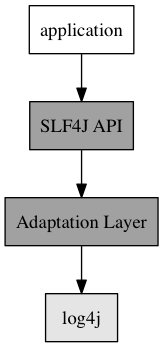
\includegraphics[width=0.5\linewidth, frame]{slf4j.png}
\caption{SLF4j Using log4j}
\label{fig:slf4jlog4j}
\end{figure}


In figure \ref{fig:slf4jlog4j} the application uses SLF4J to log. It has been bound to use log4j libraries through the adaptation layer. 

We can use the Java Logging API with SLF4J. A bit later we will swap the Java Logging API to log4j, and the code doesn't change at all.

First we will change our logging code to import the SLF4J Logger classes:
\begin{lstlisting}[language=Java]
import org.slf4j.Logger;
import org.slf4j.LoggerFactory;
\end{lstlisting}

Then we create a logger and use it to write our log messages:
\begin{lstlisting}[language=Java]
Logger logger = LoggerFactory.getLogger(this.getClass());
logger.error("Logging ERROR");
logger.warn("Logging WARN");
logger.info("Logging INFO");
logger.debug("Logging DEBUG");
\end{lstlisting}

See Appendix P on page \pageref{App:AppendixP} for the full source code for the  \texttt{ConfigLoggingEample.java} class.

In order to facilitate later swapping of the logging library, we will configure the logger in a configuration file. For Java Logging, the file is usually called \texttt{logging.properties}:
\begin{lstlisting}
handlers= java.util.logging.FileHandler, java.util.logging.ConsoleHandler
.level= FINEST

java.util.logging.FileHandler.pattern = simple.log
java.util.logging.FileHandler.limit = 50000
java.util.logging.FileHandler.count = 1
java.util.logging.FileHandler.formatter = java.util.logging.SimpleFormatter
java.util.logging.SimpleFormatter.format=%1$tb %1$td, %1$tY %1$tl:%1$tM:%1$tS %1$Tp %2$s %4$s: %5$s%n

java.util.logging.ConsoleHandler.level = FINEST
java.util.logging.ConsoleHandler.formatter = java.util.logging.SimpleFormatter
\end{lstlisting}

The source for \texttt{logging.properties} can be found in Appendix P on page \pageref{App:AppendixP}.

The first line specifies that we will use two handlers, one to log to a file and another to log to the console. The second block configures the file handler (lines 4-8). It specifies the name of the file, formatter and the format. We configure it to write to the \texttt{simple.log} file. The last block (lines 10-11)configures the console handler to use the \texttt{SimpleFormatter} also.

When we want to use the logging.properties (and Java Logging) with SLF4J, we need to trigger the runtime binding by adding a VM property to tell it where the file is when we run the program:
\begin{lstlisting}
java -cp ".:slf4j-jdk14-1.7.22.jar:slf4j-api-1.7.22.jar" -Djava.util.logging.config.file=./logging.properties org.familysearch.viitanenm.SimpleFormatterExample
\end{lstlisting}

We include the slf4j API library to the classpath (for our code) and also the binding library for Java Logging. Then we use the -Djava.util.logging.config.file Java Logging property to point to the configuration file.

The contents of the simple.log file with this configuration is:
\begin{lstlisting}
Dec 21, 2016 12:28:34 PM viitanenm.SimpleFormatterExample doIt SEVERE: Logging ERROR
Dec 21, 2016 12:28:35 PM viitanenm.SimpleFormatterExample doIt WARNING: Logging WARN
Dec 21, 2016 12:28:35 PM viitanenm.SimpleFormatterExample doIt INFO: Logging INFO
Dec 21, 2016 12:28:35 PM viitanenm.SimpleFormatterExample doIt FINE: Logging DEBUG
\end{lstlisting}

See how DEBUG translates into FINE level.

Java Logging has another formatter that we could use, XMLFormatter. We can swap to use it by changing the logging.properties file:

\begin{lstlisting}
java.util.logging.ConsoleHandler.formatter = java.util.logging.XMLFormatter
\end{lstlisting}

Now the output of the console handler changes to XML:
\begin{lstlisting}[language=XML]
<?xml version="1.0" encoding="UTF-8" standalone="no"?>
<!DOCTYPE log SYSTEM "logger.dtd">
<log>
<record>
  <date>2016-12-21T12:30:57</date>
  <millis>1482348657028</millis>
  <sequence>0</sequence>
  <logger>viitanenm.SimpleFormatterExample</logger>
  <level>SEVERE</level>
  <class>viitanenm.SimpleFormatterExample</class>
  <method>doIt</method>
  <thread>1</thread>
  <message>Logging ERROR</message>
</record>
<record>
  <date>2016-12-21T12:30:57</date>
  <millis>1482348657059</millis>
  <sequence>1</sequence>
  <logger>viitanenm.SimpleFormatterExample</logger>
  <level>WARNING</level>
  <class>viitanenm.SimpleFormatterExample</class>
  <method>doIt</method>
  <thread>1</thread>
  <message>Logging WARN</message>
</record>
<record>
  <date>2016-12-21T12:30:57</date>
  <millis>1482348657060</millis>
  <sequence>2</sequence>
  <logger>viitanenm.SimpleFormatterExample</logger>
  <level>INFO</level>
  <class>viitanenm.SimpleFormatterExample</class>
  <method>doIt</method>
  <thread>1</thread>
  <message>Logging INFO</message>
</record>
<record>
  <date>2016-12-21T12:30:57</date>
  <millis>1482348657060</millis>
  <sequence>3</sequence>
  <logger>viitanenm.SimpleFormatterExample</logger>
  <level>FINE</level>
  <class>viitanenm.SimpleFormatterExample</class>
  <method>doIt</method>
  <thread>1</thread>
  <message>Logging DEBUG</message>
</record>
\end{lstlisting}

There were no code changes made.

Log4j is another logging library that provides more functionality than Java Logging. The code itself doesn't change at all. We just configure bindings for slf4j. If we want to use log4j logging library, for example, instead of Java Logging, we just add those libraries in our classpath.

We create a log4j configuration file, \texttt{log4j2.prop\hyp{}erties}. 

The source for \texttt{log4j2.prop\hyp{}erties} can be found in Appendix P on page \pageref{App:AppendixP}.
\begin{lstlisting}
# log to the console
appender.console.type = Console
appender.console.name = STDOUT
appender.console.layout.type = PatternLayout
appender.console.layout.pattern = [%d{MM-dd-yy HH:mm:ss ZZZ}] [%p] [${hostName}] %m%n

# log to a file
appender.rolling.type = RollingFile
appender.rolling.name = RollingFile
appender.rolling.fileName = mylog.log
appender.rolling.filePattern = mylog-%d{yyyy-MM-dd-HH-mm-ss}-%i.log.gz
appender.rolling.layout.type = PatternLayout
appender.rolling.layout.pattern = [%d{MM-dd-yy HH:mm:ss ZZZ}] [%p] [${hostName}] %m%n
appender.rolling.policies.type = Policies
appender.rolling.policies.time.type = TimeBasedTriggeringPolicy
appender.rolling.policies.time.interval = 2
appender.rolling.policies.time.modulate = true
appender.rolling.policies.size.type = SizeBasedTriggeringPolicy
appender.rolling.policies.size.size=500B
appender.rolling.strategy.type = DefaultRolloverStrategy
appender.rolling.strategy.max = 5
 
logger.rolling.name = com.example.my.app
logger.rolling.level = debug
logger.rolling.additivity = true
logger.rolling.appenderRef.rolling.ref = RollingFile

#set the appender
rootLogger.level = info
rootLogger.appenderRef.stdout.ref = STDOUT
rootLogger.appenderRef.rolling.ref = RollingFile
\end{lstlisting}

Slf4j follows the \texttt{StringFormatter} syntax, but also adds some properties. In our pattern we first print the date, time, and timezone in brackets. Then we print the log level, also in brackets. Log4j provices access to the host name or IP address with the \texttt{hostName} property. We print that, and in the end our customized message from the code, followed by a new line.

Log4j automatically looks for a configuration file in the path, so we don't have to specify its location when we run the code.
\begin{lstlisting}
java -cp ".:slf4j-api-1.7.22.jar:log4j-api-2.7.jar:log4j-core-2.7.jar:log4j-slf4j-impl-2.7.jar"  org.familysearch.viitanenm.ConfigLoggingExample
\end{lstlisting}

We added the log4j libraries to the classpath. We have the slf4j api library, and three libraries from log4j; log4j api library, a core library, and a binding library (to bind slf4j and log4j). 

The output will be (with info level):
\begin{lstlisting}
[12-20-16 14:41:50 -07:00] [ERROR] [viitanenm.local] Logging ERROR
[12-20-16 14:41:50 -07:00] [WARN] [viitanenm.local] Logging WARN
[12-20-16 14:41:50 -07:00] [INFO] [viitanenm.local] Logging INFO
\end{lstlisting}

In the configuration file we defined a \texttt{RollingFile\hyp{}Appender} appender. It automatically archives the log files when they get to a specified size, or after specified time. In our example we configured it to roll when the file size is more than 500B. In practice that limit would be larger but we just want to test it.

After running the code several times, we can see the log file rolling:
\begin{lstlisting}
-rw-r--r--   87B Dec 20 14:41 mylog-2016-12-20-14-41-29-1.log.gz
-rw-r--r--   87B Dec 20 14:41 mylog-2016-12-20-14-41-33-1.log.gz
-rw-r--r--   87B Dec 20 14:41 mylog-2016-12-20-14-41-49-1.log.gz
-rw-r--r--  143B Dec 20 14:41 mylog.log
\end{lstlisting}

